\documentclass[10pt]{article}
\usepackage[a4paper,margin=20mm]{geometry}
\usepackage[T1]{fontenc}
\usepackage[utf8]{inputenc}
\usepackage{lmodern}
\usepackage{microtype}
\usepackage{amsmath,amssymb}
\usepackage{booktabs,array}
\usepackage{graphicx,float,caption}
\usepackage{enumitem}
\usepackage{xcolor}
\usepackage[unicode]{hyperref}
\usepackage{fancyhdr}

\setlist{nosep,leftmargin=*}
\hypersetup{
  colorlinks=true,
  linkcolor=black,
  urlcolor=blue,
  pdftitle={Price-Path Normality Audit for Wilder's Log-Odds RSI},
  pdfauthor={Paweł Małmyga},
  pdfsubject={Synthetic audit of additive-model normalizers on multiplicative price paths},
  pdfkeywords={RSI, log odds, log returns, multiplicative price path, normality audit}
}
\graphicspath{{figures/}}
\pagestyle{fancy}
\fancyhf{}
\lhead{Price-path normality audit}
\rhead{Computational supplement}
\cfoot{\thepage}
\setlength{\headheight}{14pt}

\title{\textbf{Price-Path Normality Audit for Wilder's Log-Odds RSI}\\[5pt]
\large Multiplicative price paths, scale calibration, and residual shape}
\author{Pawe{\l} Ma{\l}myga\\
\small Reproducible computational supplement}
\date{September 2026}
\begin{document}
\maketitle

\begin{abstract}
This computational supplement asks whether the normalization formulas derived for additive i.i.d. innovations remain useful for classical RSI when the input is a multiplicative price path. For each experiment, symmetric i.i.d. log returns are generated, exponentiated into a positive price series, and then converted to ordinary arithmetic price changes before Wilder smoothing. The same innovation path is also processed as log-price increments, which is the additive benchmark covered directly by the manuscript. The audit contains six innovation laws, five volatility levels, twelve lookbacks, and three million retained observations per law--volatility pair. At small log-return volatility the price and log-price coordinates are close. As volatility and lookback increase, the classical price coordinate develops positive skewness that variance normalization cannot remove. The manuscript normalizers remain useful scale corrections, but they are not exact pivots for the multiplicative price model and do not imply finite-sample normality.
\end{abstract}

\section{Question and scope}

The manuscript studies a generic additive input
\begin{equation}X_t=X_{t-1}+\varepsilon_t.\end{equation}
If $X_t=\log P_t$, the innovations are log returns and the interpretation is direct. Classical market RSI is usually computed from $P_t$ itself. Under
\begin{equation}P_t=P_{t-1}e^{r_t},\end{equation}
its input increments are
\begin{equation}\Delta P_t=P_{t-1}(e^{r_t}-1),\end{equation}
which are state dependent and asymmetric even when $r_t$ is symmetric. The question is therefore numerical: how accurately do the additive-model normalizers describe the classical price-RSI coordinate after this nonlinear mapping?

This is a synthetic robustness audit, not a proof for geometric price models, not a backtest, and not evidence that market returns follow any law used here. The deterministic RSI and endpoint identities remain exact on every generated path. Only the probabilistic calibration is under examination.

\section{Experimental design}

For every law and volatility level, the audit generates 3,000,000 retained observations after a burn-in of $32\times377=12{,}064$. The initial price is 10,000; a single global rescaling is applied internally to avoid floating-point overflow and cannot change RSI. The fixed seed is 20260925.

The laws are Gaussian, Laplace, and standardized Student $t_\nu$ with $\nu\in\{4,5,6,8\}$. Every innovation has variance one before multiplication by a log-return standard deviation in
\begin{equation}\{0.5\%,1\%,2\%,4\%,8\%\}.\end{equation}
The lookback grid is
\begin{equation}n\in\{2,3,5,8,13,21,35,55,89,144,233,377\}.\end{equation}
Gaussian log returns generate lognormal one-step price ratios. The Laplace and Student cases are alternative multiplicative stress models, not geometric Brownian motion. In particular, untruncated Student log returns have no positive exponential moment; those cases are finite-sample stress experiments and are not covered by the manuscript's light-tail expansion.

For each path two coordinates are calculated:
\begin{align}
L^P_{t,n}&=\log\frac{U^P_{t,n}}{D^P_{t,n}}, & U^P,D^P&\text{ smooth }(\Delta P_t)_+,(-\Delta P_t)_+,\\
L^{\log P}_{t,n}&=\log\frac{U^r_{t,n}}{D^r_{t,n}}, & U^r,D^r&\text{ smooth }(r_t)_+,(-r_t)_+.
\end{align}
The latter is the exact additive benchmark. Each coordinate is viewed under the asymptotic scale $\sqrt n/C_F$, the law-specific finite-$n$ correction, its centered version, and an empirical-variance oracle. Centering isolates shape from a finite-run location error; the oracle is diagnostic and is not a proposed usable normalizer.

\section{Diagnostics and computational validation}

The diagnostics are variance, skewness, excess kurtosis, Kolmogorov distance
from $N(0,1)$, central coverage, tail frequency, and Q--Q deviations.  For the
log-price coordinate, exact scale invariance makes the results identical across
the five volatility labels; those labels are therefore not independent
replications.

The computational validation confirms:
\begin{itemize}
\item all 2,880 expected summary rows are present with unique keys and finite
      required metrics;
\item the reported variances satisfy the algebraic scale identities to a
      maximum absolute discrepancy of $1.33\times10^{-15}$;
\item SciPy filtering agrees with a direct Wilder recursion;
\item the generated price path reconstructs the supplied log returns and is
      invariant to a global price rescaling;
\item the endpoint log-odds identity holds numerically; and
\item price RSI converges to log-price RSI in the small-volatility limit.
\end{itemize}
These checks assess implementation correctness, completeness, algebraic
consistency, and simulation stability; they are not a formal proof of the
multiplicative model.  Aggregate outputs and representative draws are provided
in the accompanying reproducibility package; see
Appendix~\ref{app:reproducibility}.

\section{Results}
\subsection{Price versus log-price benchmark}

Table~\ref{tab:mean-ks} averages Kolmogorov distance over all six laws under the centered law-specific correction. The log-price values are invariant to the volatility multiplier, as homogeneity requires. The price values increase approximately with volatility and are more sensitive at long lookbacks.

\begin{table}[ht]
\centering
\caption{Mean Kolmogorov distance over six laws.}\label{tab:mean-ks}
\begin{tabular}{rrrr}
\toprule
$\sigma_r$ & $n$ & log-price RSI & price RSI\\
\midrule
0.5\% & 55 & 0.0012 & 0.0037\\
0.5\% & 377 & 0.0036 & 0.0110\\
1.0\% & 55 & 0.0012 & 0.0072\\
1.0\% & 377 & 0.0036 & 0.0199\\
2.0\% & 55 & 0.0012 & 0.0141\\
2.0\% & 377 & 0.0036 & 0.0382\\
4.0\% & 55 & 0.0012 & 0.0282\\
4.0\% & 377 & 0.0036 & 0.0752\\
8.0\% & 55 & 0.0012 & 0.0564\\
8.0\% & 377 & 0.0036 & 0.1704\\
\bottomrule
\end{tabular}
\end{table}

\begin{figure}[H]
\centering
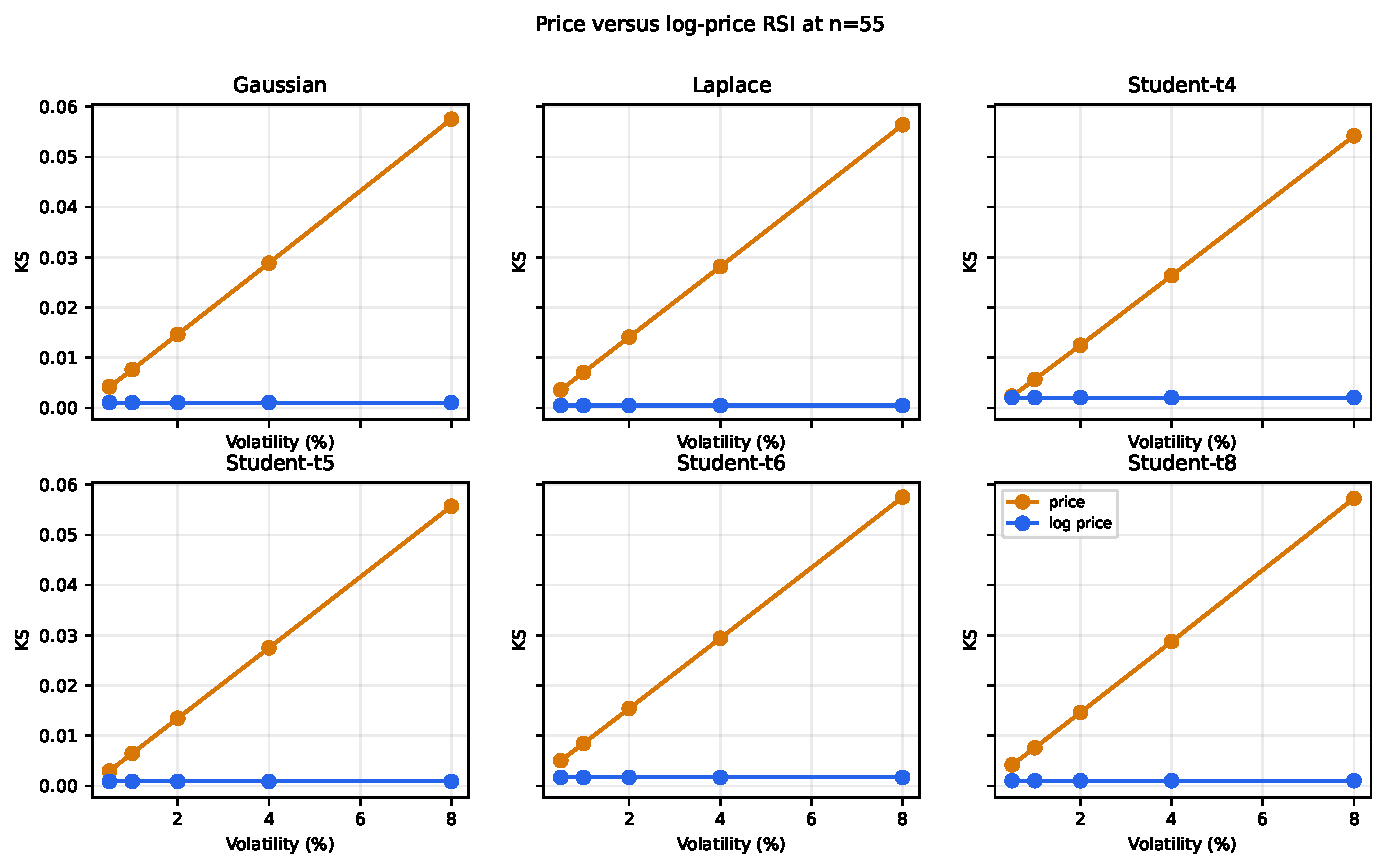
\includegraphics[height=0.335\textheight,keepaspectratio]{price_vs_log_ks_n55.pdf}
\par\vspace{-1mm}{\small (a) Lookback $n=55$.}\par\vspace{1mm}
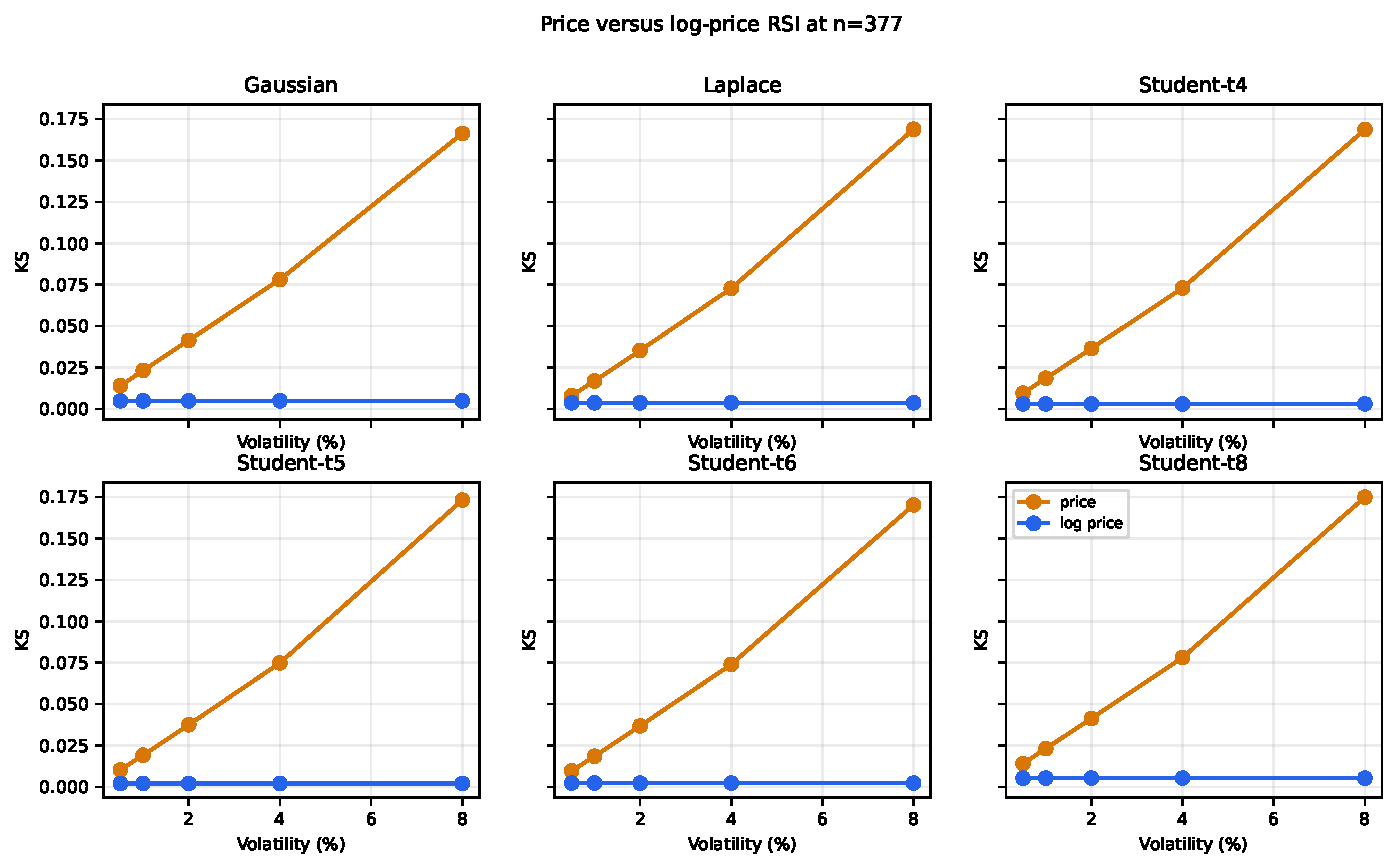
\includegraphics[height=0.335\textheight,keepaspectratio]{price_vs_log_ks_n377.pdf}
\par\vspace{-1mm}{\small (b) Lookback $n=377$.}
\caption{Classical price RSI versus the log-price benchmark.  Long memory
accumulates the multiplicative asymmetry more visibly.}
\label{fig:price-log-ks}
\end{figure}

\clearpage
\subsection{Scale correction and residual shape}

The corrected variances in Table~\ref{tab:selected} remain near one in most settings, including cases where Kolmogorov distance becomes material. Thus $g_F(n)$ can correct scale well while the resulting variable remains non-Gaussian because of skewness and tail shape.

\begin{table}[ht]
\centering\scriptsize
\caption{Selected classical price-RSI diagnostics under the centered law-specific correction. Tail is $\Pr(|Z|>3)$.}\label{tab:selected}
\begin{tabular}{lrrrrrrr}\toprule
Law & $\sigma_r$ & $n$ & Var & Skew & Excess kurt. & KS & Tail\\\midrule
Gaussian & 1\% & 55 & 1.007 & 0.120 & 0.054 & 0.0076 & 0.0031\\
Gaussian & 1\% & 377 & 1.014 & 0.318 & 0.127 & 0.0233 & 0.0041\\
Gaussian & 2\% & 55 & 1.008 & 0.228 & 0.112 & 0.0147 & 0.0036\\
Gaussian & 2\% & 377 & 1.021 & 0.595 & 0.521 & 0.0414 & 0.0067\\
Gaussian & 8\% & 55 & 1.020 & 0.879 & 1.226 & 0.0575 & 0.0096\\
Gaussian & 8\% & 377 & 1.069 & 2.264 & 7.955 & 0.1663 & 0.0212\\
Laplace & 1\% & 55 & 1.004 & 0.103 & 0.040 & 0.0071 & 0.0031\\
Laplace & 1\% & 377 & 0.989 & 0.256 & 0.116 & 0.0169 & 0.0034\\
Laplace & 2\% & 55 & 1.004 & 0.209 & 0.088 & 0.0141 & 0.0035\\
Laplace & 2\% & 377 & 0.989 & 0.538 & 0.463 & 0.0353 & 0.0058\\
Laplace & 8\% & 55 & 1.009 & 0.844 & 1.089 & 0.0564 & 0.0091\\
Laplace & 8\% & 377 & 1.005 & 2.244 & 7.766 & 0.1689 & 0.0193\\
Student-$t_4$ & 1\% & 55 & 0.999 & 0.071 & 0.056 & 0.0057 & 0.0031\\
Student-$t_4$ & 1\% & 377 & 0.987 & 0.238 & 0.066 & 0.0186 & 0.0030\\
Student-$t_4$ & 2\% & 55 & 0.999 & 0.177 & 0.089 & 0.0125 & 0.0034\\
Student-$t_4$ & 2\% & 377 & 0.985 & 0.506 & 0.341 & 0.0365 & 0.0051\\
Student-$t_4$ & 8\% & 55 & 1.000 & 0.814 & 1.044 & 0.0542 & 0.0084\\
Student-$t_4$ & 8\% & 377 & 0.974 & 2.098 & 6.414 & 0.1687 & 0.0182\\
\bottomrule\end{tabular}
\end{table}

At 0.5--1\% volatility, discrepancies are small through much of the lookback grid. At 2\%, the Gaussian price coordinate has KS 0.0147 at $n=55$ and 0.0414 at $n=377$. At 8\% and $n=377$, the laws have KS near 0.17 and pronounced positive skewness. Those are shape departures, not failures of the variance formula alone.

\begin{figure}[H]
\centering
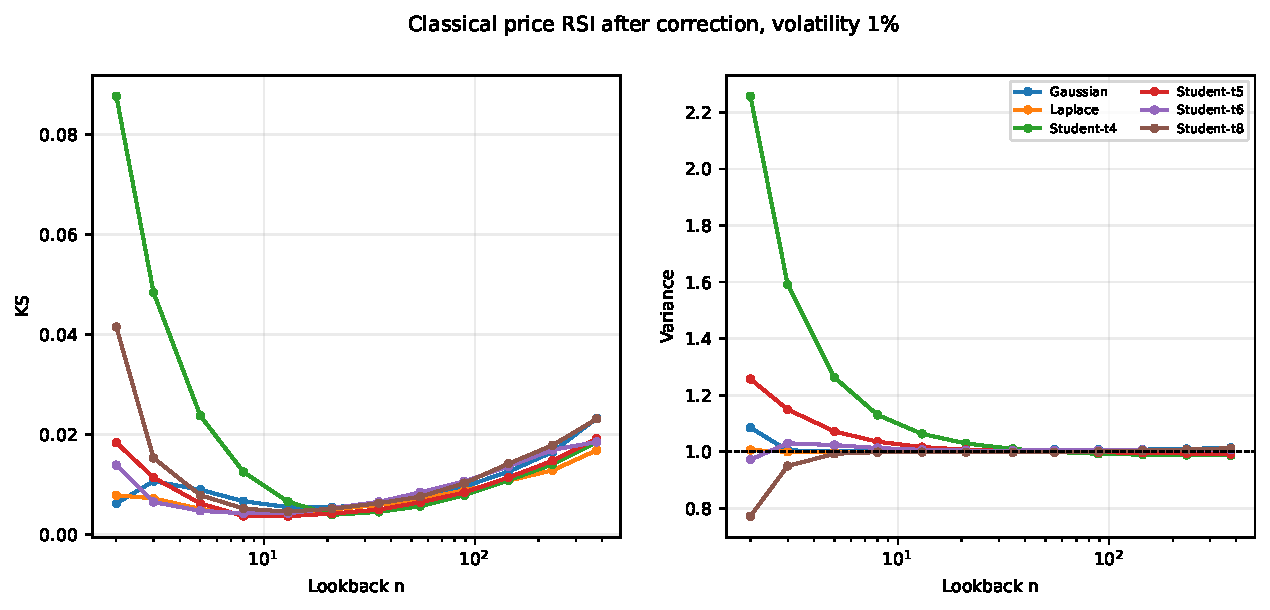
\includegraphics[width=0.92\textwidth]{corrected_price_summary_1pct.pdf}
\par\vspace{-1mm}{\small (a) Log-return volatility 1\%.}\par\vspace{2mm}
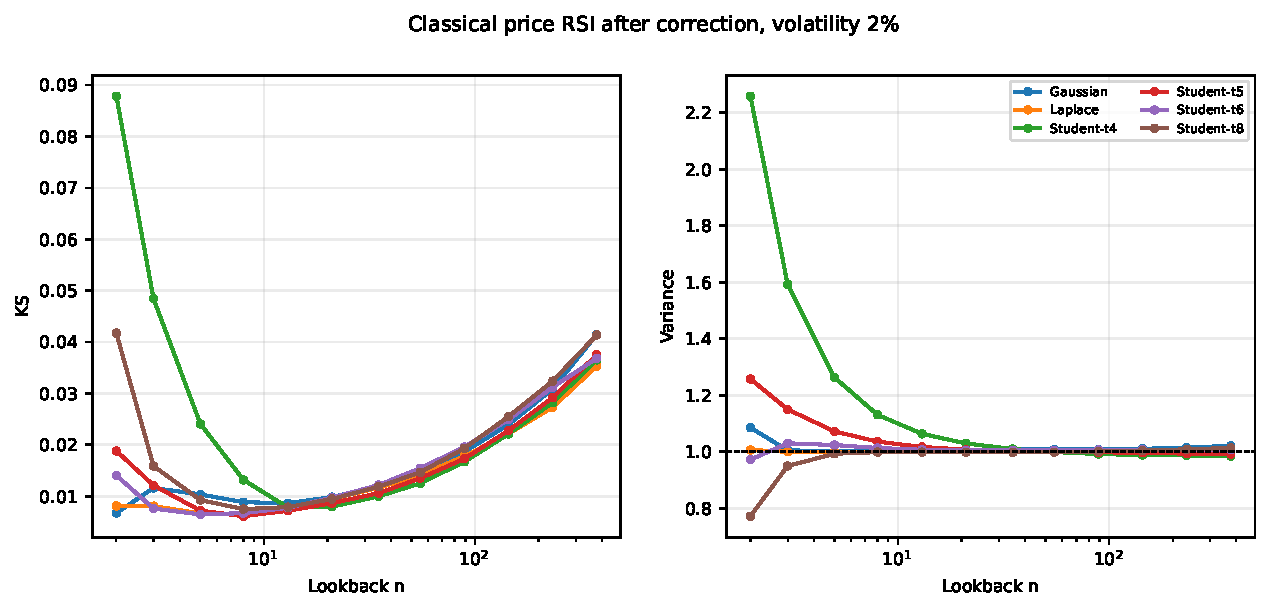
\includegraphics[width=0.92\textwidth]{corrected_price_summary_2pct.pdf}
\par\vspace{-1mm}{\small (b) Log-return volatility 2\%.}
\caption{Corrected classical price-RSI diagnostics at moderate log-return
volatility.}
\label{fig:corrected-price-summary}
\end{figure}

\clearpage
\subsection{The \texorpdfstring{$n=2$}{n=2} stress point}

The smallest lookback is deliberately retained. It shows that an asymptotic or first-shift normalizer need not be accurate merely because the innovations are standardized. For Student-$t_4$, the corrected scale equals the asymptotic scale ($K_4=0$), giving variance about 2.26 and a 4.84\% frequency beyond three standard-normal units.

\begin{table}[ht]\centering
\caption{Classical price-RSI diagnostics at $n=2$ and $\sigma_r=1\%$ under the centered law-specific correction.}
\begin{tabular}{lrrrr}\toprule
Law & Var & Excess kurt. & KS & $\Pr(|Z|>3)$\\\midrule
Gaussian & 1.085 & 0.666 & 0.0062 & 0.0083\\
Laplace & 1.006 & 0.525 & 0.0079 & 0.0059\\
Student-$t_4$ & 2.258 & 0.606 & 0.0876 & 0.0484\\
Student-$t_5$ & 1.257 & 0.625 & 0.0184 & 0.0121\\
Student-$t_6$ & 0.972 & 0.638 & 0.0139 & 0.0057\\
Student-$t_8$ & 0.772 & 0.632 & 0.0415 & 0.0026\\
\bottomrule\end{tabular}
\end{table}

For Student-$t_4$, the reported excess kurtosis is a finite-sample diagnostic;
the innovation law has no finite population fourth moment.

\section{Limitations}

\begin{itemize}
\item The study uses stationary i.i.d. synthetic log returns.  It does not test
      serial dependence, heteroskedasticity, regime changes, or empirical
      market data.
\item The additive-model normalizers are theorems for increments of the chosen
      additive input.  Their performance for classical price RSI under
      multiplicative dynamics is an empirical robustness result, not a new
      theorem.
\item The retained coordinate paths are serially dependent.  The reported
      distributional distances are descriptive Monte Carlo estimates rather
      than i.i.d. test statistics.
\item Untruncated Student log returns have no positive exponential moment and
      are used here only as finite-sample stress experiments.  In addition,
      Student $t_4$ has no finite population fourth moment, so its reported
      excess kurtosis is a sample diagnostic.
\item The audit does not identify a return law for financial data.  Gaussian,
      Laplace, and Student innovations are controlled inputs used to separate
      scale effects from residual shape effects.
\end{itemize}

\section{Conclusion}

The audit establishes a sharp distinction between exact applicability and
empirical robustness.  When the RSI input is log price and its increments
follow the assumed law, the additive-model normalizers apply directly.  For
classical price RSI, they remain useful small-return approximations: at low and
moderate synthetic volatility, much of the scale correction survives the
exponential mapping.

Variance calibration is not, however, a proof of normality.  The multiplicative
price map introduces state dependence and positive skewness that become more
visible as volatility and lookback increase.  The formulas should therefore be
described as exact or asymptotic results for additive increments and as
volatility-dependent benchmarks for ordinary price RSI.  The Student
first-shift corrections come from the companion conventional technical note
and remain outside the Lean-verified scope.

\clearpage
\appendix
\section{Selected Q--Q grids}
\label{app:qq}

The Q--Q panels superimpose classical price RSI (orange) and the log-price
benchmark (blue).  At low volatility the curves are close except in stressful
short-lookback cases.  As volatility increases, the orange curve develops a
systematic asymmetric bend while the blue benchmark stays fixed.  The first
pair contrasts Gaussian inputs at low and high volatility; the second pair
shows alternative innovation laws.

\begin{figure}[H]
\centering
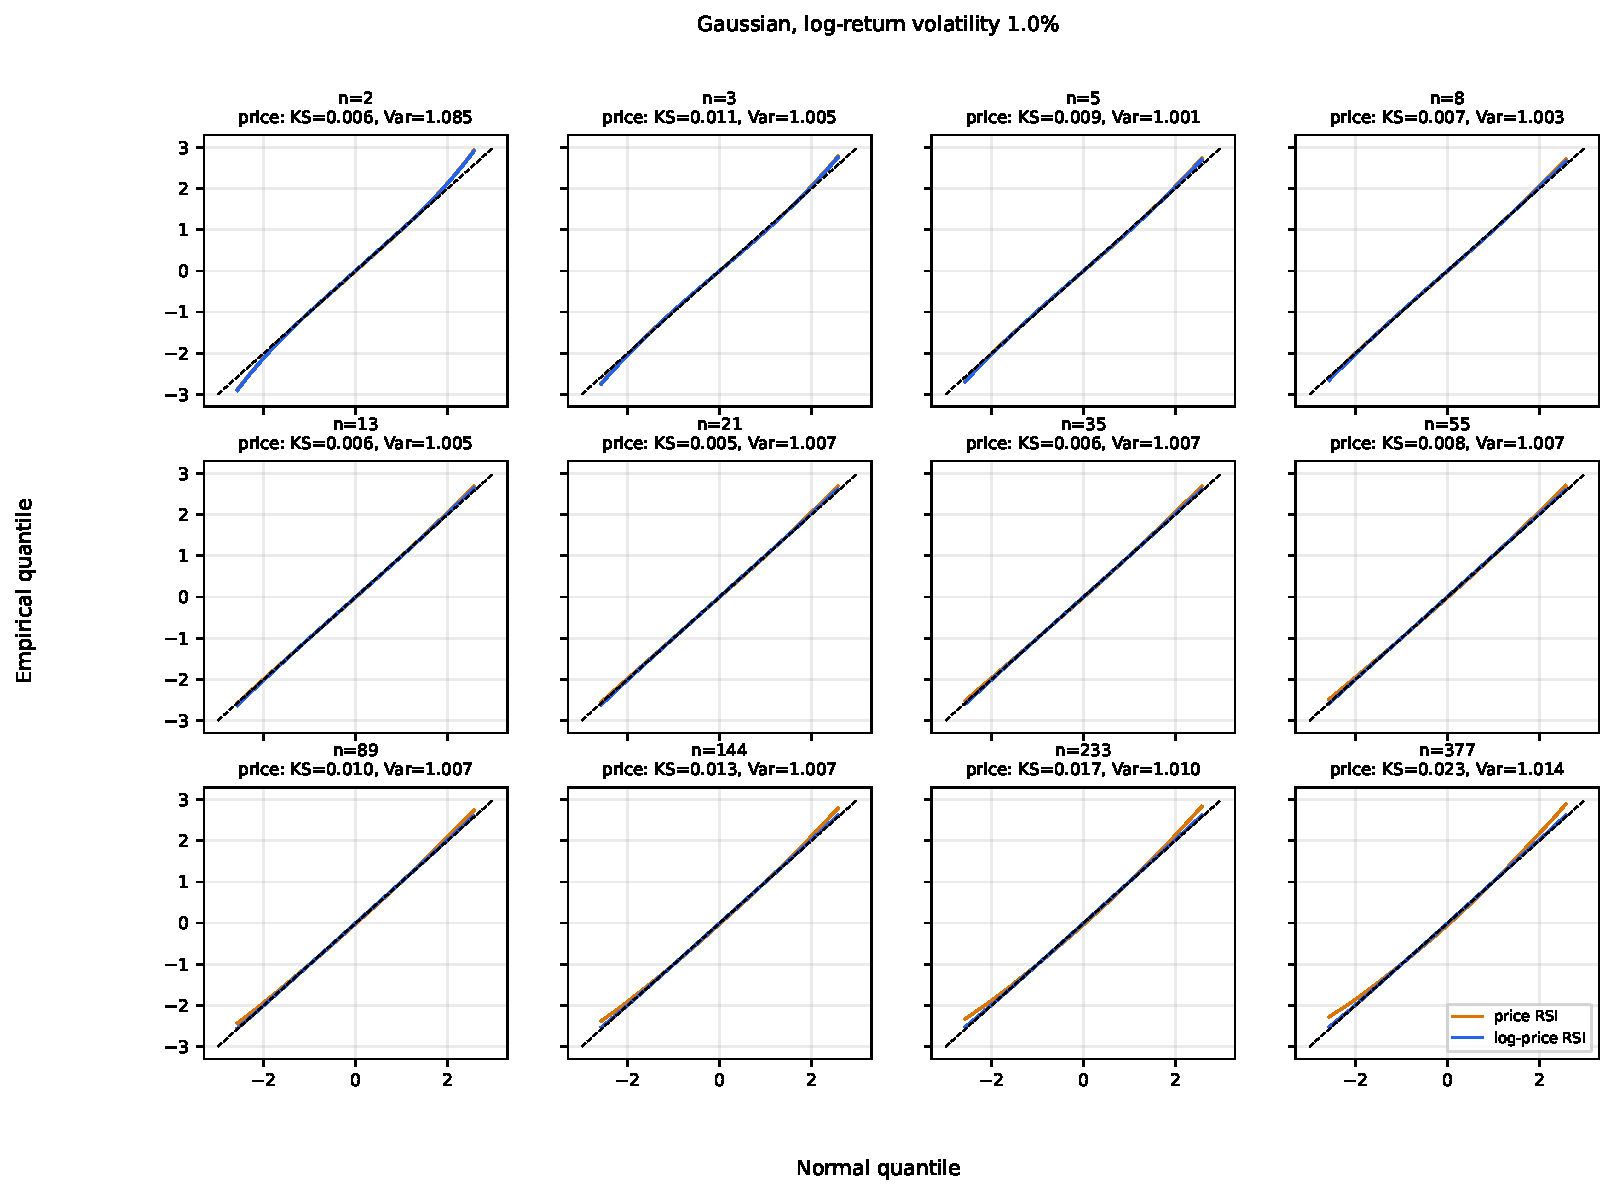
\includegraphics[height=0.35\textheight,keepaspectratio]{qq_grid_gaussian_1pct.pdf}
\par\vspace{-1mm}{\small (a) Gaussian log returns, 1\% volatility.}\par\vspace{1mm}
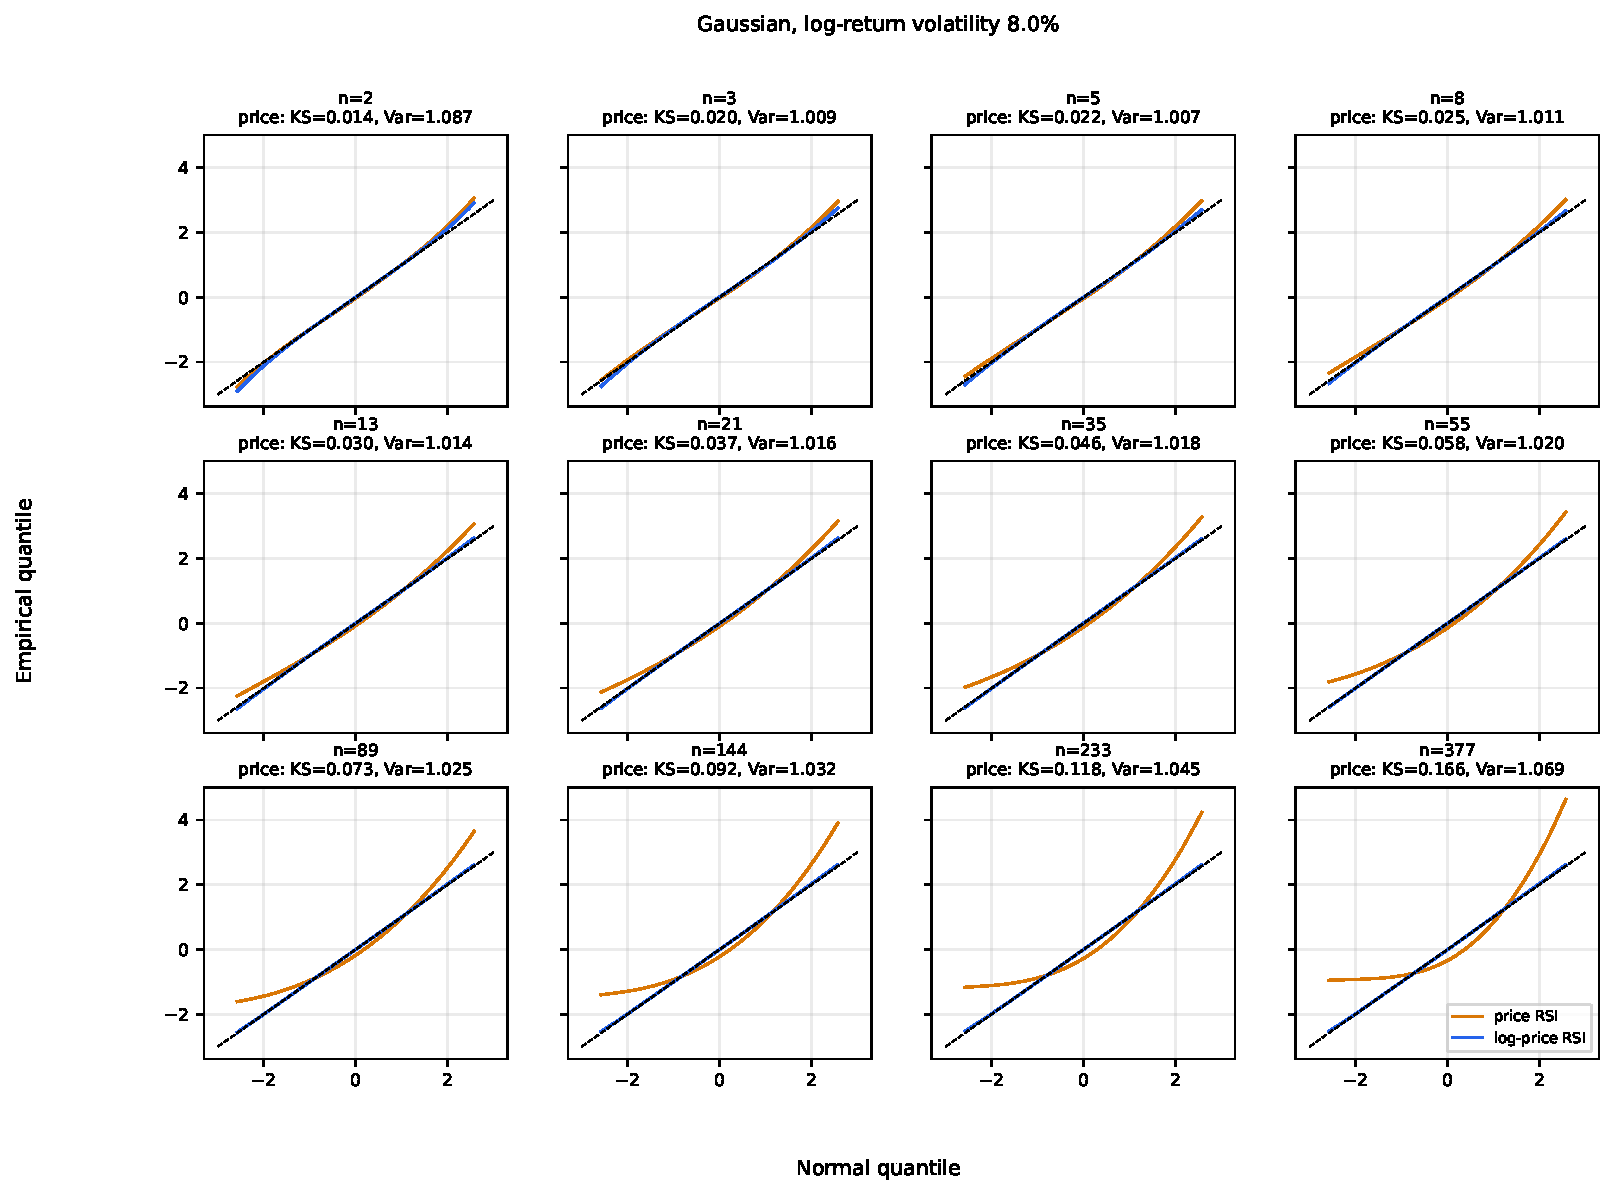
\includegraphics[height=0.35\textheight,keepaspectratio]{qq_grid_gaussian_8pct.pdf}
\par\vspace{-1mm}{\small (b) Gaussian log returns, 8\% volatility.}
\caption{Gaussian Q--Q grids.  At 8\% volatility, variance remains near one
while positive skewness invalidates a normal interpretation.}
\end{figure}

\clearpage
\begin{figure}[H]
\centering
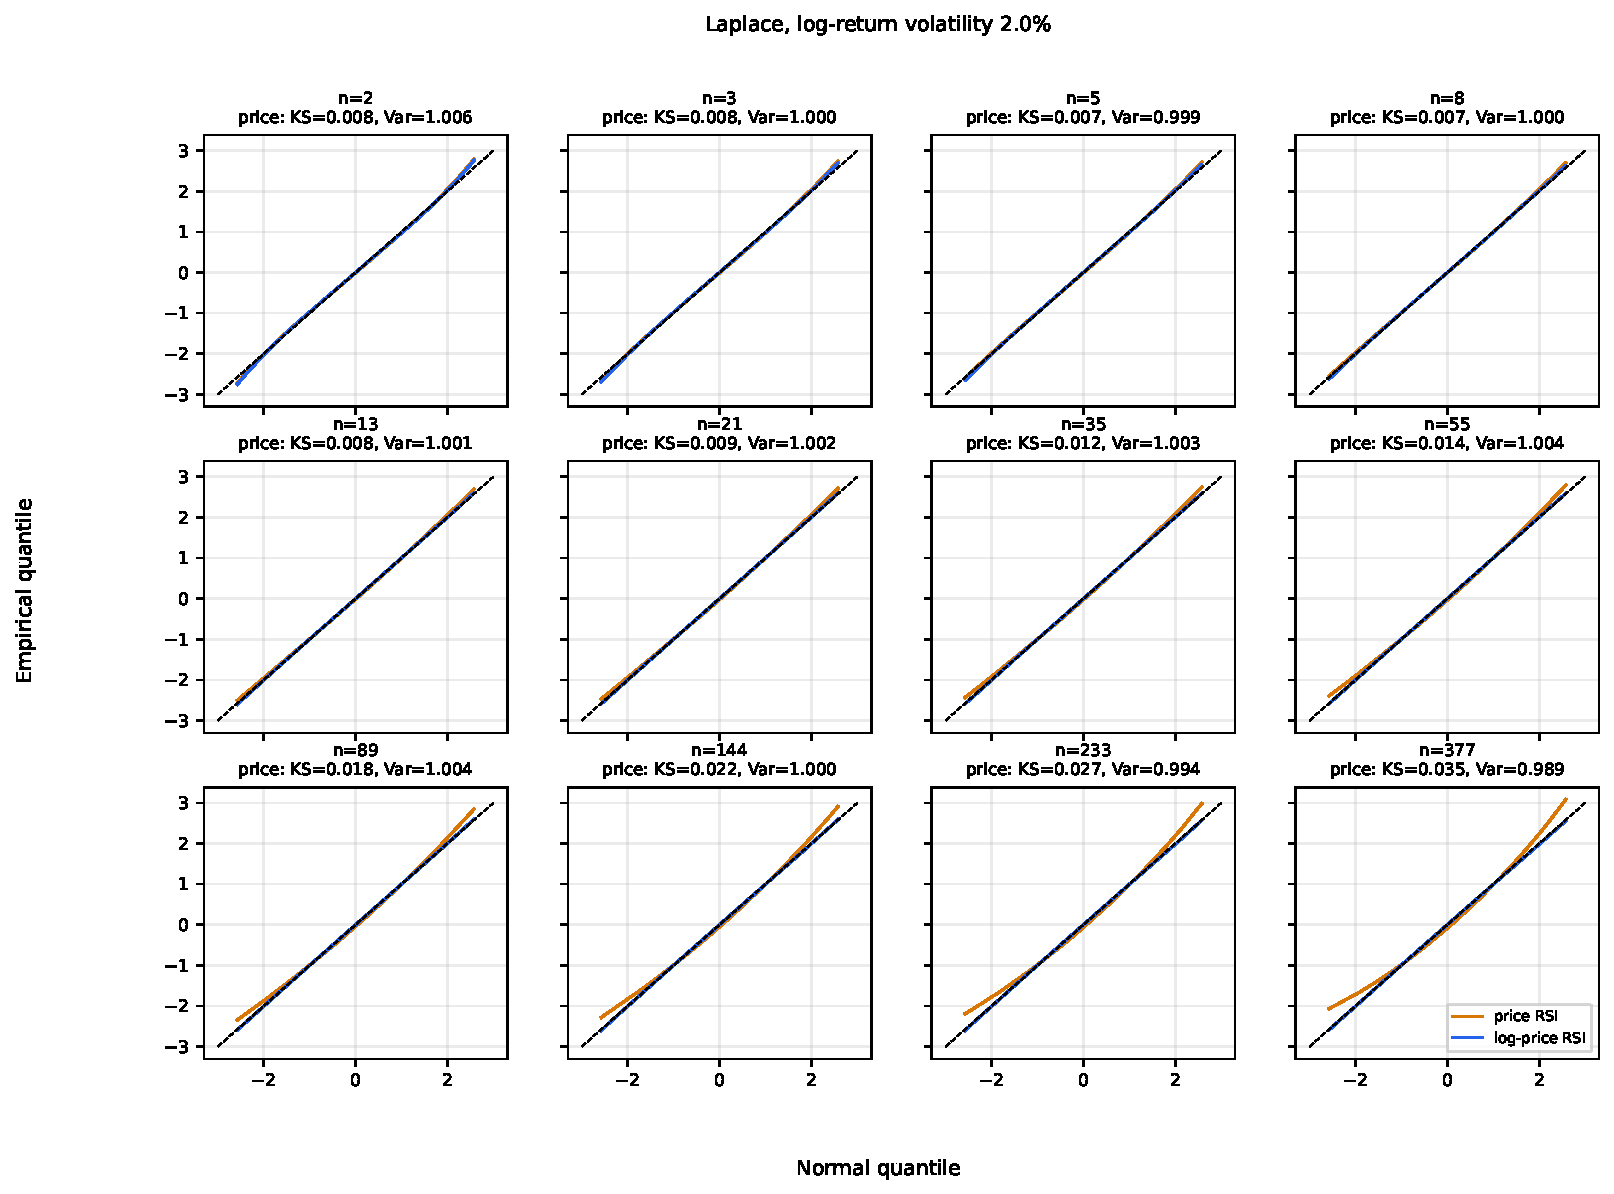
\includegraphics[height=0.375\textheight,keepaspectratio]{qq_grid_laplace_2pct.pdf}
\par\vspace{-1mm}{\small (a) Laplace log returns, 2\% volatility.}\par\vspace{1mm}
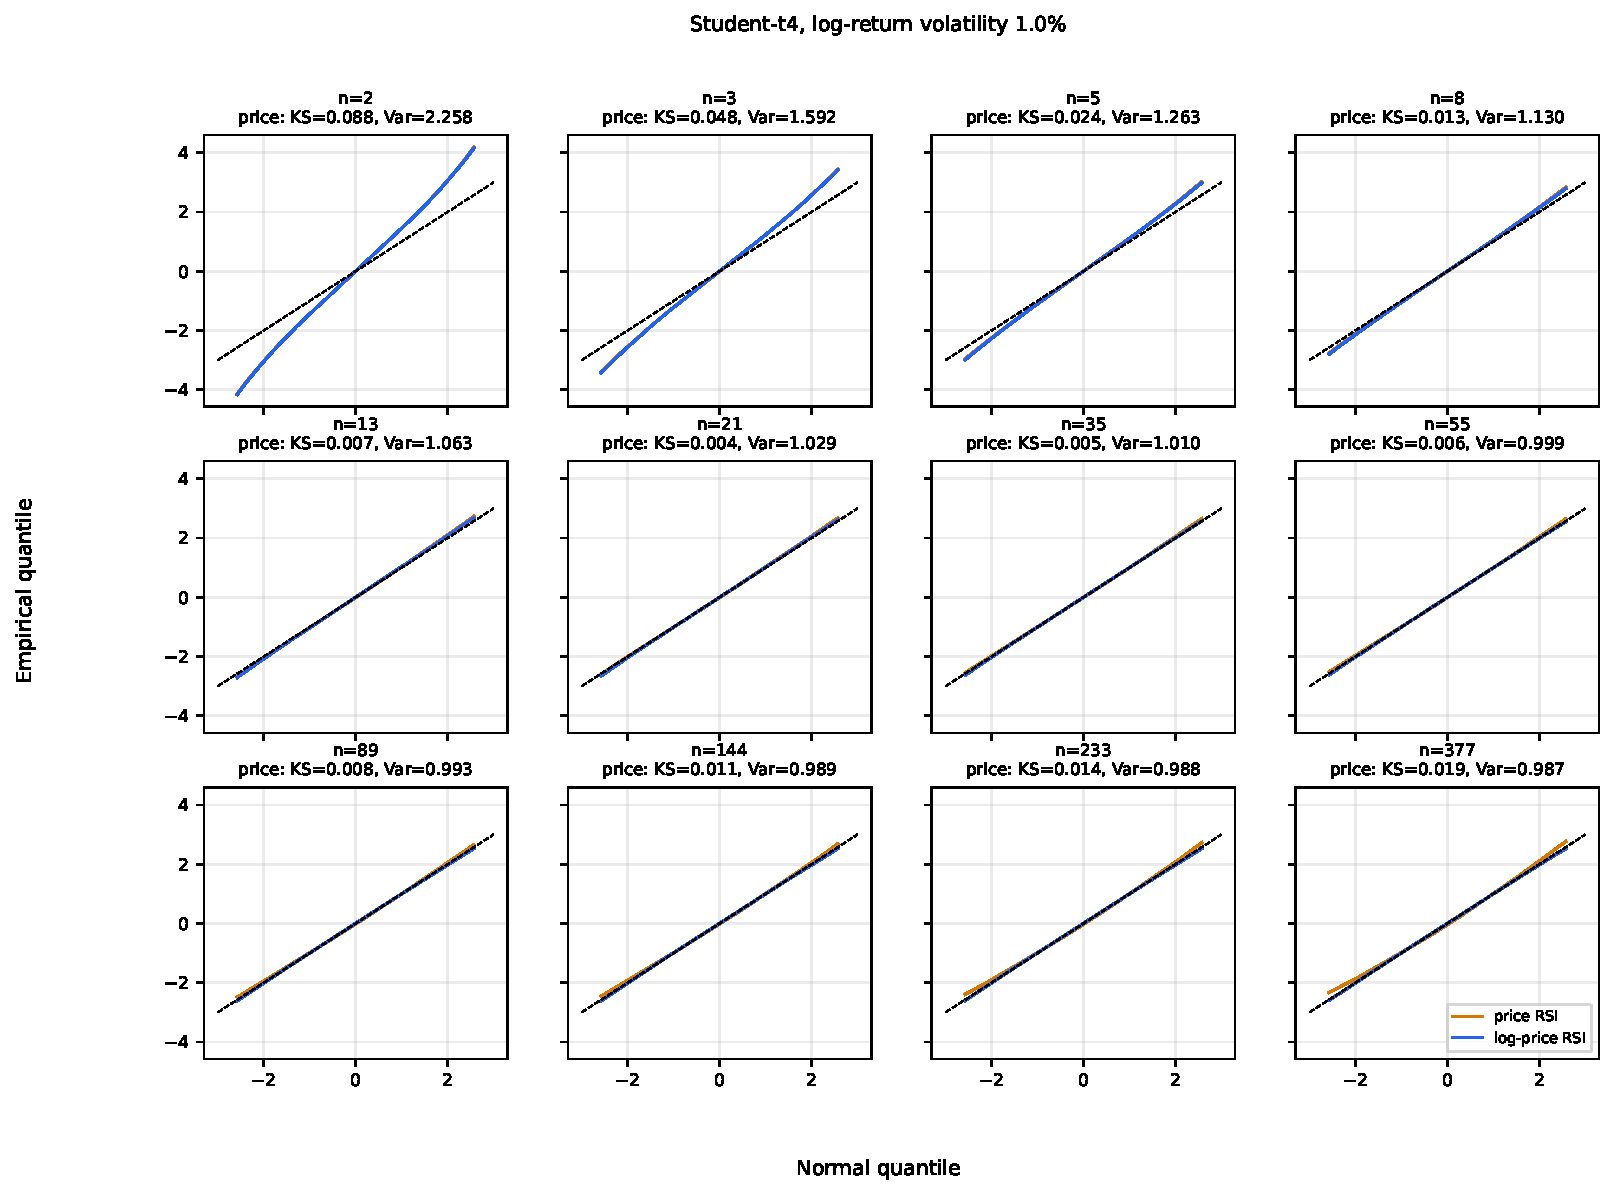
\includegraphics[height=0.375\textheight,keepaspectratio]{qq_grid_student_t4_1pct.pdf}
\par\vspace{-1mm}{\small (b) Student $t_4$ log returns, 1\% volatility.}
\caption{Laplace and Student $t_4$ Q--Q grids.  The Student $t_4$ scale error at
$n=2$ is inherited from the first-shift approximation, for which $K_4=0$.}
\end{figure}

\clearpage
\section{Reproducibility and provenance}
\label{app:reproducibility}

The archived reproducibility package contains the complete code, pinned Python
3.12 dependencies, aggregate CSV outputs, quantile and empirical-CDF grids,
histograms, block estimates, representative draws, figures, metadata, and the
implementation-validation script.  The log-price rows repeated across the five
volatility labels are identical by exact scale invariance and are not
independent replications.

On Windows, run from the repository root:
\begin{verbatim}
py -m pip install -r supplement\price_path_normality_audit\requirements.txt
py supplement\price_path_normality_audit\validate_implementation.py
py supplement\price_path_normality_audit\run_price_path_audit.py
\end{verbatim}
On Linux or macOS, use:
\begin{verbatim}
python3 -m pip install -r supplement/price_path_normality_audit/requirements.txt
python3 supplement/price_path_normality_audit/validate_implementation.py
python3 supplement/price_path_normality_audit/run_price_path_audit.py
\end{verbatim}
Published aggregate data and representative draws are sufficient for review
without repeating the complete simulation.  The \texttt{--plots-only} option
regenerates the figures from those outputs.

\medskip
\noindent
The author formulated the research question, mathematical framework, and
interpretation, and takes responsibility for the claims made in this report.
AI tools assisted with computational design, code drafting, debugging,
visualization, and editorial preparation.  Numerical results were produced by
the archived code and preserved outputs; they are not Lean-verified theorems.

\end{document}
